\documentclass[conference,9pt]{IEEEtran}
\usepackage{xcolor}
\usepackage{cite}
\usepackage{epsfig}
\usepackage{amssymb}
\usepackage{amsmath}
\usepackage{graphicx}
\graphicspath{ {./} }

\begin{document}
\title{Practical 4}

\author{
\IEEEauthorblockN{Albert Acebron}
\IEEEauthorblockA{NIU: 1458626}
}

\maketitle
\begin{abstract}
In this practical we will focus on the elimination of interferring signals through the use of adaptive filters. More concretely, we will implement the LMS algorithm and apply it on multiple scenarios with the objective of filtering unwanted signals.
\end{abstract}

\section{Implementation of LMS}
Let's start by implementing the algoritm we'll be using in this practical and doing some analysis on how it should be used.

For starters, here's a straightforward implementation of the algorithm:
\begin{verbatim}
function [H, y, e] = algoritmeLMS(d, x, P, mu)
  iterations = P:length(x);
  H=zeros(P, length(x)-P+1);
  first = -min(iterations);
  for j=iterations
    index=first+j+1;
    xn= x(j-P+1:j);
    y(index) = H(:, index)'*xn;
    e(index)=d(j)-y(index);
    H(:, index+1)=
      H(:, index)+mu*xn*conj(e(index));
  end
end
\end{verbatim}

\subsection{Analysis of values for the parameters}
Looking at the parameters needed to run the algorithm, it should be easy to tell that it's not possible to just run it only with an input signal and a reference one. Instead, we'll also have to provide $\mu$ and $P$.

$P$ just accounts for the number of coefficients that'll be used in the filter. Generally we just want to make sure to use a big enough number for it, so that the filter doesn't end up being clipped, although at the same time we'd like to keep that number as small as possible to reduce the computation required to run the algorithm. 

Later on the practical we'll explain a method on how to find a good number for this experimentally, but if we find ourselves in a situation were we have some information on what the filter will end up looking like (for example if our adaptive filter is imitating another filter) we could also use that to approximate a good guess.

On the other hand, $\mu$ is fundamentally a parameter that is tied to the size of the step taken on every iteration of the algorithm. That is, once the algorithm computes the gradient and knows what's the best direction to move forward to reach the minimum, it must also choose how big of a movement in that direction it should make, and this is determined by $\mu$ (along with how steep the gradient is at that point).

This means that, on one side, the smaller $\mu$ is, the smaller will be the steps that the algorithm takes to reach the local minimum, which will increase the total number of steps taken by the algorithm, thus making it slower. Furthermore, it's also possible that a small step size makes the algorithm get stuck in a small local minimum or, if a fixed amount of steps is used, that it is unable to reach a minimum before the algorithm finishes. On top of that, in circustances where the filter coefficients have to keep changing to adapt to changes in the environment or input signals, if the step size is too low the filter won't be able to change quickly enough to properly adapt.

On the other side, if the value of $\mu$ is too high we might end up in a situation where we overshoot the minimum and end up in the other side, which could make our algorithm slower (since we are constantly overshooting the minimum instead of closely following the steepest descent) or might even end up preventing our algorithm from converging.

In conclusion, we want to pick a value for it that it's not too small nor too big, in order to make our algorithm finish in the lowest time while also making sure it converges.

In data science it's common to vary the value of this parameter during optimization\footnote{Source: https://en.wikipedia.org/wiki/Learning\_rate}, but here we'll just set some bounds and pick a value that ensures convergence.

\subsection{Calculating the range of convergence of $\mu$}

As mentioned before, we want to use a value for $\mu$ that makes sure that the algorithm converges, but how can we know for what values that condition holds true?

In order to calculate that, we'll start by looking at equation 1.5 of the practical, which lets us calculate the new error after each consecutive step:
$$e'(n)=e(n)(1-\mu x_n^H x_n)$$

We can assert that if we want $e(n)$ to eventually converge to 0 we must make sure that the following condition is met:
$$|1-\mu x_n^H x_n|<1$$

This is because if this doesn't hold we would end up in situations where the error after applying a step is equal or larger than the one before applying the step, which means that we wouldn't be able to minimize it.

Now, if we develop the expression further, we get that:
$$0 < \mu x_n^H x_n < 1$$

And if we unroll $x_n^H x_n$ we would see how it's just a sum of multiplications between an number and it's conjugate, which hold the condition $a\cdot a*>0$, therefore $x_n^H x_n > 0$, which means that to meet the first condition two conditions must be met:
$$0 < \mu$$
$$\mu < \dfrac{1}{x_n^H x_n}$$

Finally we can compute the value of $x_n^H x_n$ with:
\begin{verbatim}
  conj(entrada')*entrada
\end{verbatim}

And, for the specific signal at hand, we will get a result of 3.8887e+13, thus a converging $\mu$ will need to be contained in:

$$0<\mu <\dfrac{1}{3.8887\cdot 10^{13}}=2.5716\cdot 10^{-14}$$

\section{Application: Recording recovery}
Let's say we find ourselves in a situation similar to the one explained in the practical, where we are tasked with recovering a recording that has been corrupted by another signal (in this case external noise) which we have also recorded alone.

In this scenario, we can recover our sound by applying our algorithm using the corrupted recording as the reference and the external noise as the input signal, and, due to the incorrelation between the external noise and the song that we want to recover we'll obtain the song as the error signal\footnote{A better explanation of how all this works is in the practical, I didn't want to just repeat it here so I've only explained the gist of it}. An explanation for how were the values of $P$ and $\mu$ picked (and why $\mu$ doesn't belong to the converge interval) is provided in the following sections.

\begin{verbatim}
  [H, y, e]=algoritmeLMS(referencia, 
    entrada, 100, 2e-11);
\end{verbatim}

Once applied, we can play the error signal and we should hear the song, which is the opening of Breaking Bad.
\begin{verbatim}
  sound(e, Fs);
\end{verbatim}

\subsection{Improvements on the algorithm}
When applied to the signal at hand, the extracted sound (equivalent to the error inside the algorithm) turned out to be very noisy in the beginning. I believe this is caused by the fact that the filter coefficients are all initialized to 0, which makes it perform badly until it has gone through a few samples and optimized itself.

To prevent this noisyness, I added another iteration of the algorithm where the last filter coefficients are used as the initialized parameters of the first filter, which succeeded in making the initial filter better and it reduced the initial noise to barely anything, thus improving the result.
\begin{verbatim}
function [H, y, e] = algoritmeLMS(d, x, P, mu)
  iterations = P:length(x);
  H=zeros(P, length(x)-P+1);
  first = -min(iterations);
  for k=1:2
    for j=iterations
      index=first+j+1;
      xn= x(j-P+1:j);
      y(index) = H(:, index)'*xn;
      e(index)=d(j)-y(index);
      H(:, index+1)=
        H(:, index)+mu*xn*conj(e(index));
    end
    H(:, 1) = H(:, first+max(iterations));
  end
end
\end{verbatim}

\subsection{Value of $\mu$}

Note that the $\mu$ that we've used is outside the convergence range calculated on the first sections. This is because, after trying experimentally with multiple posssible values of $\mu$, we achieved the best results with values close to $10^{-11}$, whereas the values contained in our convergency range didn't work well.

This is because smaller step sizes don't manage to reach the minimum within the number of iterations we are using in our algorithm ($2|samples|$), as all movements are very small\footnote{I've verified this experimentally by increasing the number of iterations of the algorithm and checking that even with a small $\mu$, it works fine}, whereas with larger steps the minimum is reached but, because these are outside the convergency range, it's likely that we don't end up in the absolute minimum and instead end up in it's surroundings (and if the step size is too large we could end up overshooting our minimum completely, but this doesn't happen for values around $\mu=10^{-11}$).

Overall, this can be fixed by increasing the total number of iterations of the algorithm from 2 to 20 (in the case of using $\mu=2\cdot 10^{-14}$, if we were to use a smaller value we'd need to increase it even further), which can be done by changing this line:
\begin{verbatim}
  for k=1:2
\end{verbatim}

to this one:
\begin{verbatim}
  for k=1:20
\end{verbatim}

After making this change we can apply the algorithm with $\mu=2\cdot 10^{-14}$ and it will work fine (theoretically the end results should also be better, but I can't tell the difference in terms of sound). All in all, this is a classical example of a computation tradeoff, where if we spend more computation power we can guarantee convergency and make sure we reach the minimum.

\subsection{Number of filter coefficients}

The number of coefficients of the filter was picked through the following steps:

1. Initially pick a random number

2. Apply the algorithm and check that the sound works fine

3. Plot the coefficients to make sure we are not clipping part of the filter.

Let's go ahead and plot the coefficients of the last iteration of the filter (with $P=100$):

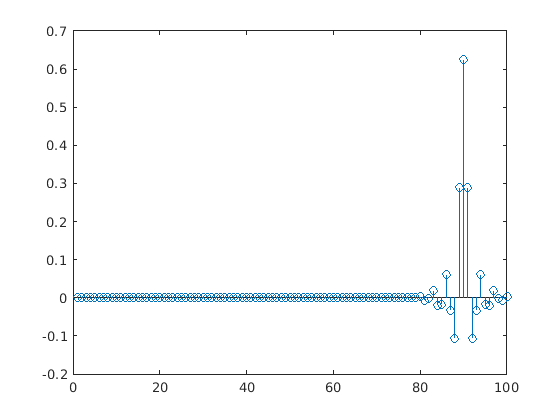
\includegraphics[scale=0.6]{coef.png}

In this case, looking at the plot of the filter it became clear that only 30 values or so are used for it, as the rest are set to 0, so it's quite clear that with 100 coefficient there is no clipping. If we were to re-calculate the filter using $P=25$, we'd get the following plot instead:

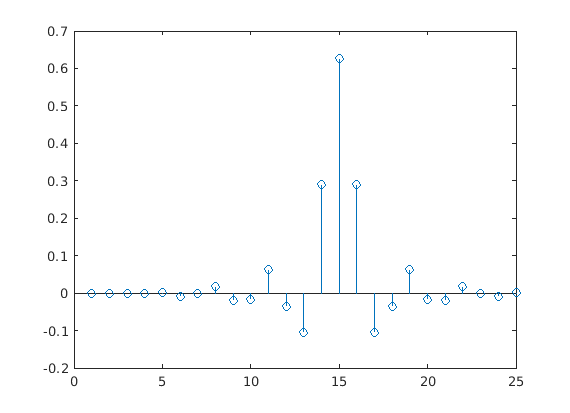
\includegraphics[scale=0.6]{coef25.png}

So, as we can see, it would be possible to make this number smaller, which would decrease the computation power required for the algorithm, but right now the computations don't take much time so there's no need to do that.

Note that these coefficients have been obtained from the second algorithm provided, the one that uses two iterations to improve the initial filter estimation.








\section{Application: Removal of interferring signal}
In this scenario we have received a signal that has the following periodogram:

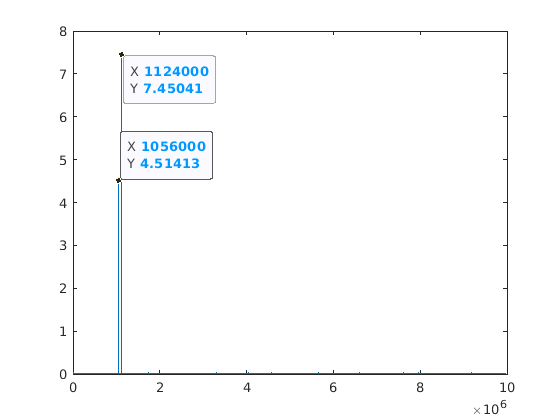
\includegraphics[scale=0.6]{perio.png}

Where the pulse at 1.124 MHz is an unwanted inteferring signal and the one at 1.05 MHz is the one we are really interested in.

Given that both pulses are concentrated on a very narrow frequency range and we'll need to filter very selectively in order to remove the one we don't want, we'll be using a notch filter.

With that in mind, we'll start by constructing the notch filter and applying it directly. Afterwards, we'll apply the algorithm we developed before to the filtered results and see if it's possible for the adaptive filter to end up simulating the results we got with the notch one.

\subsection{Construction of the notch filter}
In order to calculate the transfer function of our notch filter we could start by combining equations (1.2) and (1.3) from the practical B, which gets us:

$$\frac{\sum b_k z^{-k}}{1 + \sum a_k z^{-k}} = K\frac{1-2cos(\omega_{int})z^{-1} + z^{-2}}{1- 2rcos(\omega_{int})z^{-1}+r^2z^{-2}}$$

So if we solve this equation for the coefficients we'll get that:
$$b_0=1$$
$$b_1=-2cos(\omega_{int})$$
$$b_2=1$$
$$a_0=1$$
$$a_1=-2rcos(\omega_{int})$$
$$a_2=r^2$$

Using this we can calculate the value of $K$:
$$K=\frac{1 + a_1+a_2}{b_0+b_1+b_2}=\frac{1-2rcos(\omega_{int})+r^2}{1-2cos(\omega_{int})+1}$$

If we now take a look at the periodogram of the practical 3:

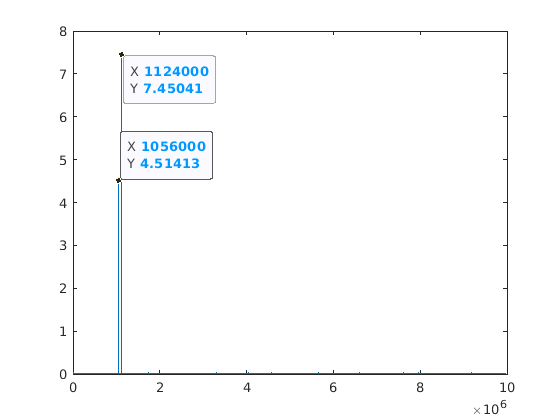
\includegraphics[scale=0.6]{perio.png}

We can calculate $\omega_{int}$ using the frequency of the inteferring signal:
$$\omega_{int}=\frac{2\pi \cdot 1.124 MHz}{10 MHz} = 0.7062$$

And then proceed to graph the impulsional response of the filter (initially using $r=1.5$):

\begin{verbatim}
  wint = 0.7062;
  r=1.5;
  K=(1-2*r*cos(wint)+r^2)/(1-2*cos(wint)+1);
  w=0:pi/1000:pi;
  z=exp(j*w);
  H=K*(1-2*cos(wint)*z.^(-1)+z.^(-2))
   ./(1-2*r*cos(wint)*z.^(-1)+r^2*z.^(-2));
  % Plot
  plot(w, 10*log(abs(H)));
\end{verbatim}

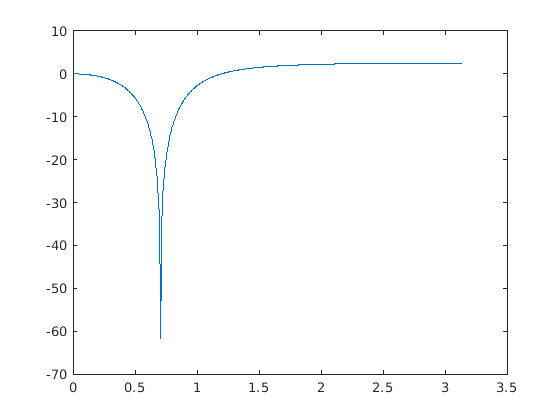
\includegraphics[scale=0.6]{filter-response.png}

And if we now overlap it with the tones of the signal:

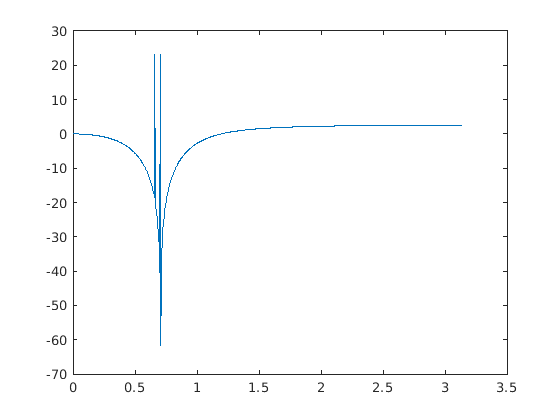
\includegraphics[scale=0.6]{complete-filter-res.png}

As we can see, the filter is correctly filtering our interferring signal, but the other signal is also getting caught up in it. To fix that we'll set $r=1.15$:

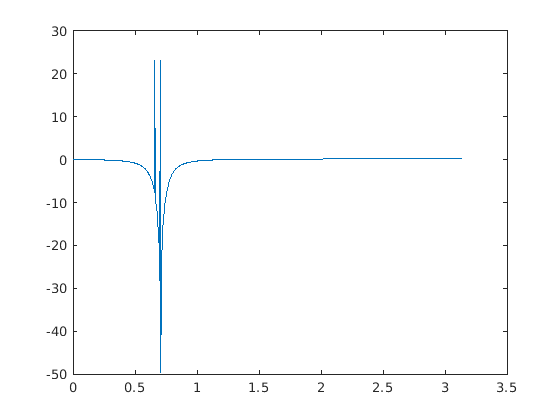
\includegraphics[scale=0.6]{r1-1.png}

Now the filter is much more selective and, although it still reduces our wanted signal, the reduction is much lower.

\subsection{Filtering with the notch filter}
Let's apply the notch filter we constructed to get rid of the unwanted signal, to do so we'll calculate the filter coefficients and use filter():
\begin{verbatim}
  r=1.15
  a=[r^2, -2*r*cos(wint), 1]
  b=[1, -2*cos(wint), 1]*K
  filtered=filter(b, a, RxSignal)
  per = compute_periodogram(filtered)
  plot(linspace(0, 1e7, length(per)), per)
\end{verbatim}

Which results in a signal that has the following periodogram:

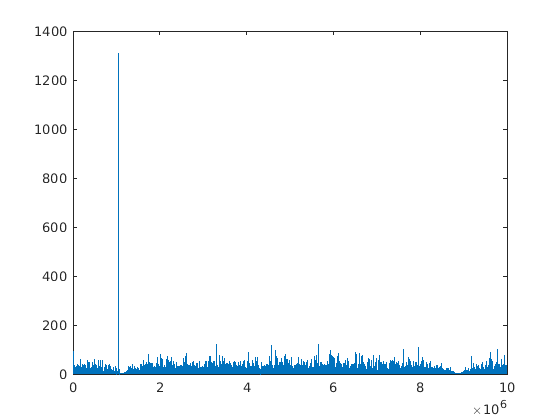
\includegraphics[scale=0.6]{filtered.png}

As we can appreciate, the unwanted signal has been completely removed.

\subsection{Imitation with adaptive filter}
Next, we'll try to use an adaptive filter to simulate the notch filter developed before. This will be done by using the filtered signal from before as our reference signal $d(n)$ and minimizing the error $e(n)$:

\begin{verbatim}
  [Hf, y, e]=algoritmeLMS(filtered, RxSignal,
     60, 1e-5);
  per = compute_periodogram(y)
  plot(linspace(0, 1e7, length(per)), per)
\end{verbatim}

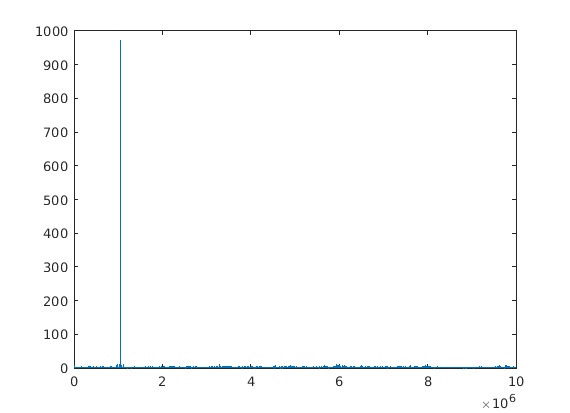
\includegraphics[scale=0.6]{filtered-lms.png}

The signal at the interferring frequency has been removed, so the filter is working well.

If we now proceed to graph the frequency response of the last iteration of the adaptive filter (we've chosen the last iteration because it should be the best one), we'll see the following result:

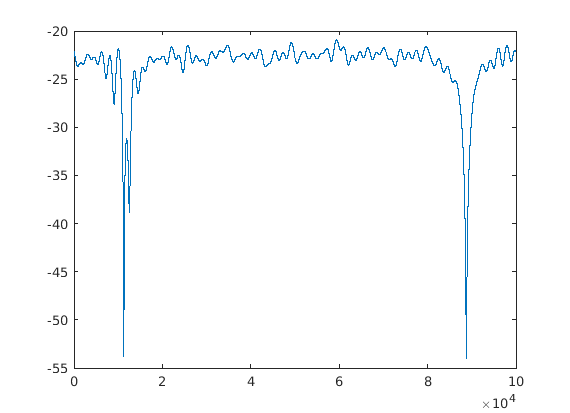
\includegraphics[scale=0.6]{freq-response.png}

As we can expect, the filter has evolved to heavily reduce the signal at the interferring frequency, but also surprisingly we see a notch on the other side of the spectrum that mitigates signals at that frequency. The reason behind this second notch is that, if we look closely at the periodogram of the filtered signal we got previously, we'll see that the frequencies on the same spot at the right end of the spectrum got reduced as well, so LMS has replicated that part of the filtering as well by adding a second notch there.

If we want to dig deeper, the reason why frequencies on that spot in the right side of the spectrum got reduced is that, in the construction of the notch filter, we apply the cosine function to $w_{int}$, which represents the inteferring frequency. $cos$ has the property that $cos(x)=cos(-x)$ so we'll get the same filter whether our interferring frequency is $w_{int}$ or $2\pi-w_{int}$, meaning that the filter must mitigate both of those frequencies to work effectively.

\subsection{Comparing impulsional responses among filters}
Now we'll proceed to compare the impulsional response of the adaptive filter with the one it is imitating, the notch filter.

To do so, we'll need to get the impulsional response of our notch filter, which we'll obtain by applying the definition of impulsional response, that is the output signal of a system through which a dirac delta has been sent.

So we'll just construct a dirac delta (that has a number of points equal to the amount of coefficients used in LMS, as the practical requires the response to have the same amount of points) and apply our filter to it with filter(), as we did previously.

\begin{verbatim}
  d=zeros(60, 1);
  d(1)=1e5;
  resp=filter(b, a, d);
  plot(resp)
\end{verbatim}

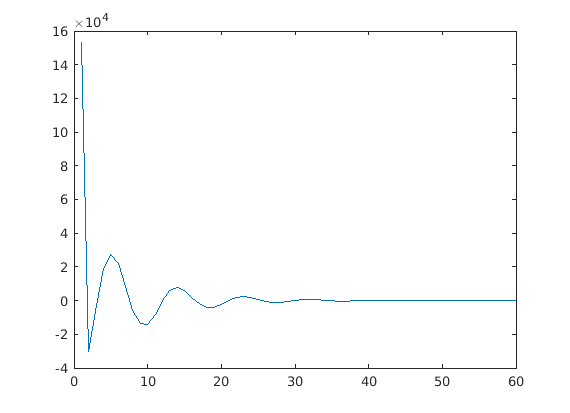
\includegraphics[scale=0.6]{imp-resp.png}

Let's now compare this result with the impulsional response of the filter derived from LMS (concretely the one from the last iteration). In this case the coefficients already represent the impulsional response so we can just use those directly:
\begin{verbatim}
  plot(abs(Hf(:,length(Hf))))
\end{verbatim}

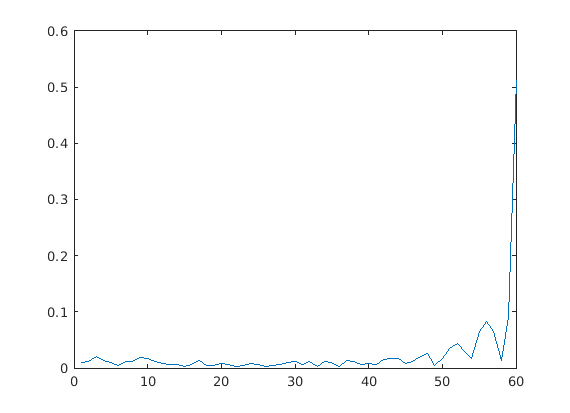
\includegraphics[scale=0.6]{im-lms.png}

If we compare this against the absolute value of the impulsional response of the notch filter:

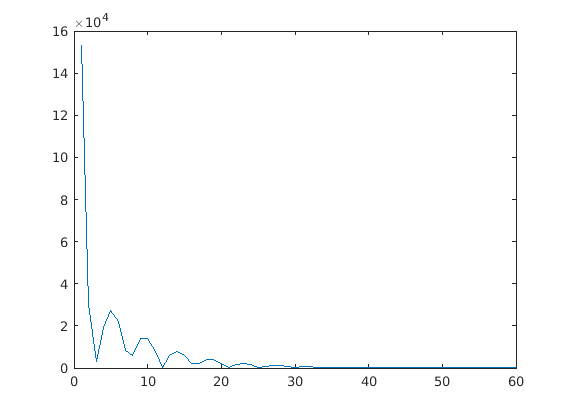
\includegraphics[scale=0.6]{im-abs.png}

We can appreciate that, ignoring the scale difference (this is just caused by the value of the delta that we applied, which is arbitrary since we can't create a perfect delta and are forced to use an approximation), both impulse responses are extremely similar but are time reversed against the other.

These being similar is what we would expect, as, after all, the LMS-derived filter is just trying to imitate the notch filter, so if it does it's job well the coefficients of the filter should end up being extremely similar, as the filter is replicated.

The time reversal is unexpected though, but it's existence can be explained with the time reversal property of the fourier transform, which says that if the fourier transform is applied to a time-reversed function the resulting function will be a conjugated version of what we would get if we applied the transform to a non-time-reversed version of the same function, in other words $F(h(-t))=H*(f)$.

Now, when we compute the periodogram we are calculating $|F(h)|^2$, which provides the same results whether F is conjugated or not ($|H|^2$=$|H*|^2$), so putting together these two facts we can conclude that the periodogram will be the same if our filter has been time reversed ($|F(h(-t))|^2=|H*|^2=|H|^2=|F(h(t))|^2$). Thus, the property of reducing the interferring signal will hold true if the impulsional response has been time-reversed.

Putting it all together, we conclude that the impulsional responses of the two filters are extremely similar and fulfill it's objectives well, which is what we wanted since the LMS-based filter is imitating the other one.

\section{Analysis of the evolution of LMS}
In this final section we'll analyze how the filter used by the LMS evolves through optimization.

To do so we'll look at how the adaptive filter changes through the 4942 iterations it goes as as part of the LMS algorithm, so we'll look at the first coefficient of the filter in several of these and compare it against the one in the notch filter it's trying to imitate in order to trace it's evolution through time:

\begin{verbatim}
  notch=resp(1)
  it=zeros(5,1)
  it(1)= Hf(60,10)-notch
  it(2)=Hf(60,100)-notch
  it(3)=Hf(60,500)-notch
  it(4)=Hf(60,2000)-notch
  it(5)=Hf(60,end)-notch
  plot([10, 100, 500, 2000, length(Hf)],
    abs(it))
\end{verbatim}

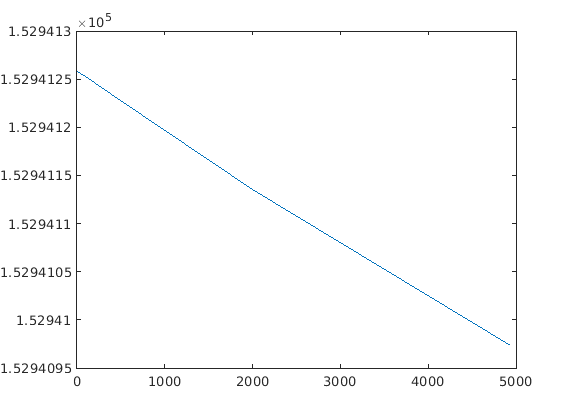
\includegraphics[scale=0.6]{error-evolution.png}

As we can see, with an increase in iterations the LMS filter gets closer to the notch one. This makes sense, since LMS is just optimizing it's filter to become similar to the other one, so the more iterations the algorithm runs the better the optimization will be and thus the closer the filter will be to the one it's trying to imitate, driving the error to zero.

\subsection{Impact of $\mu$ on evolution}
An interesting experiment to try here is to apply the LMS algorithm with multiple possible values of $\mu$, because that defines the step size used in the optimization, thus we should theoretically see that if we increase the step size the speed at which the error goes down increases (with a few caveats, for example if the step size ends up continuously overshooting the minimum we might end up with a lower rate of descent or no convergence), as each iteration will move a larger distance towards the minimum.

This can be seen in the following graph, which contains multiple values of $\mu$ (blue: 1e-5, red: 1e-4, yellow: 1e-10):

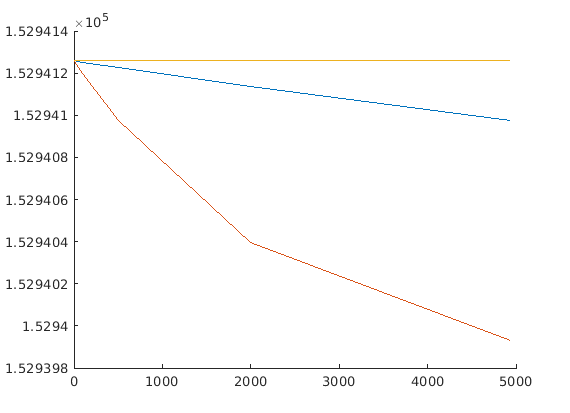
\includegraphics[scale=0.6]{mus.png}

The previous graph proves that what we theorized holds true and higher learning rates/values of $\mu$ lead to faster reduction of the error.

\section{Conclusion}
We've managed to implement the LMS algorithm and successfully apply it in multiple scenarios, including the removal of the signal that was interferring with our GNSS signal, thus completing the objective of this practical.

\section{Appendix}
\subsection{Plot coefficients of last iteration of filter}
\begin{verbatim}
  stem(H(:, length(H)))
\end{verbatim}

\subsection{Add tones to filter response graph}
\begin{verbatim}
  H(round(1124000/5e6*length(H)))=10;
  H(round(1056000/5e6*length(H)))=10;
\end{verbatim}

\subsection{Graph frequency response of adaptive filter}
\begin{verbatim}
  plot(10*log10(compute_periodogram(Hf(:,
   length(Hf)))))
\end{verbatim}

\subsection{Plot absolute impulsional response}
\begin{verbatim}
  plot(abs(resp))
\end{verbatim}

\subsection{Plot error through iterations for multiple $\mu$}
Repeat the following code for multiple values of mu:
\begin{verbatim}
  mu = 1e-5
  [Hf, y, e]=algoritmeLMS(filtered, RxSignal, 60, mu);
  notch=resp(1)
  it=zeros(5,1)
  it(1)= Hf(60,10)-notch
  it(2)=Hf(60,100)-notch
  it(3)=Hf(60,500)-notch
  it(4)=Hf(60,2000)-notch
  it(5)=Hf(60,end)-notch
  plot([10, 100, 500, 2000, length(Hf)], abs(it))
\end{verbatim}




\end{document}


